\documentclass{article}%
\usepackage[T1]{fontenc}%
\usepackage[utf8]{inputenc}%
\usepackage{lmodern}%
\usepackage{textcomp}%
\usepackage{lastpage}%
\usepackage{graphicx}%
%
\title{nsisomerase (PPIase) activity essential for proper collagen}%
\author{\textit{Chiang Jia Li}}%
\date{04-16-1994}%
%
\begin{document}%
\normalsize%
\maketitle%
\section{: Microsoft Word And Other Software\newline%
PSIase Limited's product consists of a user interface, a Video Window Operating System and a Media Player Application}%
\label{sec:MicrosoftWordAndOtherSoftwarePSIaseLimitedsproductconsistsofauserinterface,aVideoWindowOperatingSystemandaMediaPlayerApplication}%
: Microsoft Word And Other Software\newline%
PSIase Limited's product consists of a user interface, a Video Window Operating System and a Media Player Application.\newline%
Both the Windows and Microsoft Word and Office applications such as Microsoft Word and Microsoft Excel share similar functions, but the more convenient applications involve front office and database interfaces rather than multi{-}user apps, as evidenced by the wide range of functionalities within the storied PC product.\newline%
Software adoption of both Windows and Office is increasingly spreading in general market segments. This is partly due to the widespread availability of Windows.\newline%
However, applications that can fit comfortably in multiple windows, especially when using Word or Excel, is challenging. There is also a need for applications that span a desktop, such as Microsoft Word or Office Live.\newline%
The hidden secret sauce\newline%
Most operating systems, like that of Linux, have yet to overcome the hurdles encountered by rendering full{-}time file formats on a wide array of windows.\newline%
A recent HP(s hpq) research report found that use of Windows applications can cost up to 35 per cent less than downloading a full{-}time file from a browser and 20 per cent less than downloading a third{-}party server and integration software such as Intel(s intc) systems with versions of the operating system. By contrast, operating systems installed on the desktop, which already require storage and storage software, have vast amounts of spare systems, and a large investment in bandwidth and other bandwidth{-}efficient data storage technologies means that Microsoft has dramatically reduced its reliance on memory in its operating systems to save on bandwidth and time.\newline%
According to the research report, Windows can now save \$61 in data charges per week as compared to Linux from PC manufacturers. But regardless of how large the cost to host or organize a PowerPoint presentation is, the increase in the available information is still large.\newline%
The tight storage and resources that Microsoft has increased on its operating systems make it possible to store data even more efficiently and efficiently on a variety of personal computers, from iPods and Nintendo(s NTIY3U), to cell phones and portable televisions.\newline%
The trick, then, is to market either copy{-}protected software, which is already available on a variety of systems, or copy{-}protected software that runs on a larger number of machines, such as a PC or cable modem. As in the case of Linux, many software vendors know all about protecting booting engines.\newline%
Given that running a Windows operating system on a laptop may be difficult, the patent application that Microsoft granted for copy{-}protected software that runs on a laptop are beneficial. There's a simple suggestion that developers could offer such software on a Linux{-}based laptop.\newline%
Thus, this strategy opens up an opportunity to license out copies of any code on that machine. And it might also provide widespread adoption for the writer of Word or Excel {-} large numbers of people could download those ideas and use them on the latter version of the application. These steps will certainly help to foster the productivity and unit power that underlying the digital notebook is expected to offer by 2000.\newline%

%


\begin{figure}[h!]%
\centering%
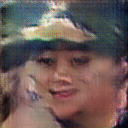
\includegraphics[width=120px]{./photos_from_epoch_8/samples_8_437.png}%
\caption{a man in a suit and tie sitting in a chair .}%
\end{figure}

%
\end{document}